
\section{Wednesday for MAT3040}\index{Wednesday_lecture}
\subsection{Jordan Normal Form}
\begin{theorem}[Jordan Normal Form]\label{The:9:3}
Suppose that $T:V\to V$ has minimial polynomial 
\[
m_T(x) = \prod_{i=1}^k(x-\lambda_i)^{e_i},
\]
then there exists a basis $\mathcal{A}$ such that
\[
(T)_{\mathcal{A},\mathcal{A}}=\diag(J_1,\dots,J_\ell),
\]
where each block $J_i$ is a square matrix of the form
\[
%J_{i} = \begin{pmatrix}
%\mu&1&\cdots&0\\
%0&\mu&\cdots&0\\
%0&\cdots&\ddots&1\\
%0&\cdots&\ddots&\mu
%\end{pmatrix}
J_i = 
\begin{bmatrix}
\mu_i & 1            & \;     & \;  \\
\;        & \mu_i    & \ddots & \;  \\
\;        & \;           & \ddots & 1   \\
\;        & \;           & \;     & \mu_i       
\end{bmatrix}.
\]
\end{theorem}
\begin{remark}
By primary decomposition theorem,
\[
V=V_1\oplus \cdots\oplus V_k,\quad
\text{where }
V_i = \ker((T - \lambda_iI)^{e_i}),\ i=1,\dots,k,
\]
and each $V_i$ is $T$-invariant.

We pick basis $\mathcal{B}_i$ for each subspace $V_i$, then 
$\mathcal{B}:=\cup_{i=1}^k\mathcal{B}_i$ is a basis of $V$, 
and
\[
(T)_{\mathcal{B},\mathcal{B}}
=
\begin{pmatrix}
(T\mid_{V_1})_{\mathcal{B}_1,\mathcal{B}_1}&0&\cdots&0\\
0&(T\mid_{V_2})_{\mathcal{B}_2,\mathcal{B}_2}&\vdots&0\\
\vdots&\ddots&\vdots&\vdots&\\
0&\cdots&\vdots&(T\mid_{V_k})_{\mathcal{B}_k,\mathcal{B}_k}
\end{pmatrix}
\]
with $m_{T\mid_{V_i}}(x) = (x-\lambda_i)^{e_i}$.
\end{remark}

Therefore, it suffices to show the Jordan normal form holds for the linear operator $T$ with minimal polynomial $m_T(x) = (x-\lambda)^e$.
%
% the theorem for 
%for $m_T(x) = (x-\lambda)^e$, since then we can get
%\[
%(T\mid_{V_i})_{\mathcal{B}_i,\mathcal{B}_i}
%=
%\diag(\bm J_1,\dots,\bm J_{\ell_i}),
%\]
%where 
%\[
%J_{a}
%=
% \begin{pmatrix}
%\mu&1&\cdots&0\\
%0&\mu&\cdots&0\\
%0&\cdots&\ddots&1\\
%0&\cdots&\ddots&\mu
%\end{pmatrix}
%\]


Firstly, we consider the case where the minimal polynomial has the form $x^m$:
\begin{proposition}\label{pro:9:5}
Suppose $T:V\to V$ is such that $m_T(x) = x^m$, then the theorem~(\ref{The:9:3}) holds, i.e., there exists a basis $\mathcal{A}$ such that
\[
(T)_{\mathcal{A},\mathcal{A}}=\diag(\bm J_1,\dots,\bm J_{\ell}),
\]
where each block $J_i$ is a square matrix of the form
\[
J_{i}
=
\begin{bmatrix}
0& 1            & \;     & \;  \\
\;        & 0    & \ddots & \;  \\
\;        & \;           & \ddots & 1   \\
\;        & \;           & \;     &0
\end{bmatrix}.
\]
\end{proposition}
\begin{proof}
\begin{itemize}
\item
Suppose that $m_T(x) = x^m$, then it is clear that
\[
\{0\}:=\ker(T^0)\le \ker(T)\le\ker(T^2)\le\cdots\le\ker(T^m):=V
\]
Furthermore, we have $\ker(T^{i-1})\subsetneqq\ker(T^i)$ for $i=1,\dots,m$:
Note that $\ker(T^{m-1})\subsetneqq\ker(T^m):=V$ due to the minimality of $m_T(x)$;
and $\ker(T^{m-2})\subsetneqq\ker(T^{m-1})$ since otherwise for any $\bm x\in\ker(T^m)$, 
\[
T^{m-1}(T\bm x)=\bm0\implies
T\bm x\in\ker(T^{m-1})=\ker(T^{m-2})
\implies
T^{m-2}(T\bm x)=T^{m-1}(\bm x)=\bm0,
\]
i.e., $\bm x\in\ker(T^{m-1})$, which contradicts to the fact that $\ker(T^{m-1})\subsetneqq\ker(T^m)$.
Proceeding this trick sequentially for $i=m,m-1,\dots,1$, we proved the disired result.
\item
Then construct the quotient space $W_i = \ker(T^i)/\ker(T^{i-1})$ and define $\mathcal{B}_i'$ to be a basis of $W_i$:
\[
\mathcal{B}_i' = \{a_1^i+\ker(T^{i-1}),\dots,a_{\ell_i}^i+\ker(T^{i-1})\}
\]
Construct $\mathcal{B}_i = \{a_1^i,\dots,a_{\ell_i}^i\}$, then we claim that $B := \cup_{i=1}^m\mathcal{B}_i$ forms a basis of $V$:
\begin{itemize}
\item
First proof the case $m=2$ first: let $U\le V$ ($\dim(V)<\infty$), and $\mathcal{B}_1=\{a_1^1,\dots,a_{k_1}^1\}$ be a basis of $U$, and
\[
\mathcal{B}_2'=\{a_1^2+U,\dots,a_{k_2}^2+U\}
\]
be a basis of $V/U$.
Then to show the statement suffices to show that 
\[
\bigcup_{i=1}^2\{a_1^i,\dots,a_{k_i}^i\}\text{ forms a basis of }V.
\]
It's clear that $\cup_{i=1}^2\{a_1^i,\dots,a_{k_i}^i\}$ spans $V$.
Furthermore, $\dim(V)=\dim(U)+\dim(V/U)=k_1+k_2$, i.e.,  $\cup_{i=1}^2\{a_1^i,\dots,a_{k_i}^i\}$ contains correct amount of vectors.
The proof is complete.
\item
This result can be extended from $2$ to general $m$, thus the claim is shown.
\end{itemize}
\item
For $i<m$, consider the set $S_i=\{T(\bm w_j)+\ker(T^{i-1})\mid \bm w_j\in B_{i+1}\}$. Note that 
\begin{itemize}
\item
Since $T^{i+1}(\bm w_j)=\bm0$, $T^i(T(\bm w_j))=\bm0$, we imply $T(\bm w_j)\in\ker(T^i)$, i.e., $S_i\subseteq W_i$.
\item
The set $S_i$ is linearly independent:
consider the equation
\[
\sum_jk_j(T(\bm w_j)+\ker(T^{i-1}))=\bm0_{W_i}
\Longleftrightarrow
T\left(\sum_jk_j\bm w_j\right)+\ker(T^{i-1})=\bm0_{W_i}
\]
i.e.,
\[
T\left(\sum_jk_j\bm w_j\right)\in\ker(T^{i-1})
\Longleftrightarrow
T^{i-1}(T(\sum_jk_j\bm w_j))=\bm0_V,
\]
i.e., $\sum_jk_j\bm w_j\in\ker(T^i)$,
i.e.,
\[
\sum_jk_j\bm w_j +\ker(T^i) = \bm0_{W_{i+1}}
\Longleftrightarrow
\sum_jk_j(\bm w_j+\ker(T^i))=\bm0_{W_{i+1}}.
\]
Since $\{\bm w_j+\ker(T^i),\ \forall j\}$ fomrs a basis of $W_{i+1}$, we imply $k_j=0,\forall j$.
\end{itemize}
From $\mathcal{B}_{i+1}$ we construct $S_i$, which is linearly independent in $W_i$. Therefore, we imply $|T(\mathcal{B}_{i+1})|\le|\mathcal{B}_i|$ for $\forall i<m$ (why?).
\item
Now we start to construct a basis $\mathcal{A}$ of $V$:
\begin{itemize}
\item
Start with $\mathcal{B}_m':=\{u_1^{m}+\ker(T^{m-1}),\dots,u_{\ell_m}^m+\ker(T^{m-1})\}$, and $\mathcal{B}_m=\{u_1^m,\dots,u_{\ell_m}^m\}$.
\item
By the previous result, 
\[
\{T(u_1^m)+\ker(T^{m-2}),\dots,T(u_{\ell_m}^m)+\ker(T^{m-2})\}
\]
is linear independent in $W_{m-1}$.
By basis extension, we get a basis $\mathcal{B}_{m-1}'$ of $W_{m-1}$, and let
\[
\mathcal{B}_{m-1} = \{T(u_1^m),\dots,T(u_{\ell_m}^m)\}\cup\xi_{m-1}
\]
where $\xi_{m-1}:=\{u^{m-1}_{1},\dots,u^{m-1}_{\ell_{m-1}}\}$
\item
Continue the process above to obtain $\mathcal{B}_{m-2},\dots,\mathcal{B}_1$, and $\cup_{i=1}^m\mathcal{B}_i$ forms a basis of $V$:
\begin{figure}[H]
\centering
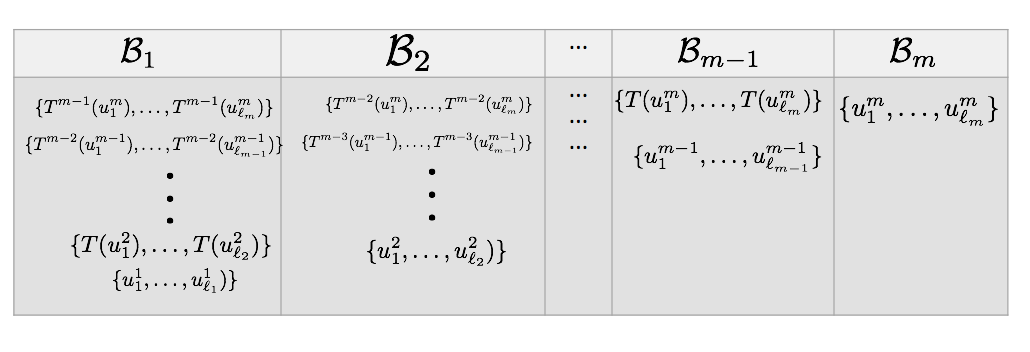
\includegraphics[width=1\textwidth]{week9/p_2}
\end{figure}
\item
Now construct the ordered basis $\mathcal{A}$:
\[
\mathcal{A}=
\left\{
\begin{array}{ccccc}
T^{m-1}(u_1^m)&\cdots&T^{2}(u_1^m)&T(u_1^m)&u_1^m\\
\vdots&\vdots&\ddots&\vdots&\vdots\\
T^{m-1}(u_{\ell_m}^m)&\cdots&T^{2}(u_{\ell_m}^m)&T(u_{\ell_m}^m)&u_{\ell_m}^m\\
\;&T^{m-2}(u_1^{m-1})&\cdots&T(u_1^{m-1})&u_1^{m-1}\\
\;&\vdots&\ddots&\vdots&\vdots\\
\;&T^{m-2}(u_{\ell_{m-1}}^{m-1})&\cdots&T(u_{\ell_{m-1}}^{m-1})&u_{\ell_{m-1}}^{m-1}\\
\;&\;&\vdots&\ddots&\vdots\\
\;&\;&\;&\;&u_1^1\\
\;&\;&\;&\;&\vdots\\
\;&\;&\;&\;&u_{\ell_1}^1\\
\end{array}
\right\}
\]
\item
Then the diagonal entries of $(T)_{\mathcal{A},\mathcal{A}}$ should be all zero, since
\[
T(T^{i-1}(u_{j}^i))=T^{i}(u_j^i)=0,\forall i=1,\dots,m, j=1,\dots,\ell_{i},
\]
and every entry on the superdiagonal is 1:

\begin{figure}[H]
\centering

\includegraphics[width=0.7\textwidth]{week9/p_3}
\caption{Illustration for $(T)_{\mathcal{A},\mathcal{A}}$}
\end{figure}
\end{itemize}



\end{itemize}
\end{proof}

Then we consider the case where $m_T(x) = (x-\lambda)^e$:
\begin{corollary}
Suppose $T:V\to V$ is such that $m_T(x) = (x-\lambda)^e$, then the theorem~(\ref{The:9:3}) holds, i.e., there exists a basis $\mathcal{A}$ such that
\[
(T)_{\mathcal{A},\mathcal{A}}=\diag(J_1,\dots,J_{\ell}),
\]
where each block $J_i$ is a square matrix of the form
\[
J_{i}
=
\begin{bmatrix}
\lambda& 1            & \;     & \;  \\
\;        & \lambda    & \ddots & \;  \\
\;        & \;           & \ddots & 1   \\
\;        & \;           & \;     &\lambda
\end{bmatrix}.
\]
\end{corollary}

\begin{proof}
Suppose that $m_T(x) = (x-\lambda)^e$. Consider the operator $U:=T-\lambda I$, then $m_U(x) = x^e$.

By applying proposition~(\ref{pro:9:5}), 
\[
(U)_{\mathcal{A},\mathcal{A}}=\diag(\bm J_1,\dots,\bm J_\ell),
\]
where 
\[
J_i=\begin{bmatrix}
0& 1            & \;     & \;  \\
\;        & 0    & \ddots & \;  \\
\;        & \;           & \ddots & 1   \\
\;        & \;           & \;     &0
\end{bmatrix}.
\]
Or equivalently,
\[
(T)_{\mathcal{A},\mathcal{A}}-\lambda(I)_{\mathcal{A},\mathcal{A}}=\diag(\bm J_1,\dots,\bm J_\ell)
\]
i.e.,
\[
(T)_{\mathcal{A},\mathcal{A}}=\diag(\bm K_1,\dots,\bm K_\ell),
\]
where
\[
\bm K_i=\begin{bmatrix}
\lambda& 1            & \;     & \;  \\
\;        & \lambda    & \ddots & \;  \\
\;        & \;           & \ddots & 1   \\
\;        & \;           & \;     &\lambda
\end{bmatrix}
\]
\end{proof}
\begin{remark}
The Jordan Normal Form Theorem~(\ref{The:9:3}) follows from our arguments using the primary decomposition.
\end{remark}


\begin{corollary}
Any matrix $A\in M_{n\times n}(\mathbb{C})$ is similar to a matrix of the Jordan normal form
\[
\diag(\bm J_1,\dots,\bm J_\ell).
\]
\end{corollary}

\subsection{Inner Product Spaces}
\begin{definition}[Bilinear]
Let $V$ be a vector space over $\mathbb{R}$.
A bilinear form on $V$ is a mapping
\[
F:V\times V\to\mathbb{R}
\]
satisfying
\begin{enumerate}
\item
$F(\bm u+\bm v,\bm w) = F(\bm u,\bm w)+F(\bm v,\bm w)$
\item
$F(\bm u,\bm v+\bm w)= F(\bm u,\bm v)+F(\bm u,\bm w)$
\item
$F(\lambda\bm u,\bm v)=\lambda F(\bm u,\bm v)=F(\bm u,\lambda\bm v)$
\end{enumerate}
We say 
\begin{itemize}
\item
$F$ is symmetric if $F(\bm u,\bm v)=F(\bm v,\bm u)$
\item
$F$ is non-degenerate if $F(\bm u,\bm w)=\bm0$ for $\forall \bm u\in V$ implies $\bm w=0$
\item
$F$ is positive definite if $F(\bm v,\bm v)>0$ for $\forall\bm v\ne\bm0$
\end{itemize}
\end{definition}


\begin{remark}
If $F$ is positive-definite, then $F$ is non-degenerate:
Suppose that $F(\bm v,\bm v)>0,\forall\bm v\ne\bm0$.
If we have $F(\bm u,\bm w)=0$ for any $\bm u\in V$, then in particular, when $\bm u=\bm w$, we imply $F(\bm w,\bm w)=0$. By positive-definiteness, $\bm w=\bm0$, i.e., $F$ is non-degenerate.
\end{remark}




















